\documentclass[a4paper,12pt]{article}
%%%%%%%%%%%%%%%%%%%%%%%%%%%%%%%%%%%%%%%%%%%%%%%%%%%%%%%%%%%%%%%%%%%%%%%%%%%%%%%%%%%%%%%%%%%%%%%%%%%%%%%%%%%%%%%%%%%%%%%%%%%%%%%%%%%%%%%%%%%%%%%%%%%%%%%%%%%%%%%%%%%%%%%%%%%%%%%%%%%%%%%%%%%%%%%%%%%%%%%%%%%%%%%%%%%%%%%%%%%%%%%%%%%%%%%%%%%%%%%%%%%%%%%%%%%%
\usepackage{eurosym}
\usepackage{vmargin}
\usepackage{amsmath}
\usepackage{graphics}
\usepackage{epsfig}
\usepackage{subfigure}
\usepackage{fancyhdr}
\usepackage{listings}
\usepackage{framed}
\usepackage{graphicx}
\usepackage{amsmath}
\usepackage{chngpage}
%\usepackage{bigints}

%\setcounter{MaxMatrixCols}{10}

\begin{document}
	\large
	\section{Speeding up visualizations with WebGL}
When visualizing large datasets with Bokeh, the interaction can become rather slow. To counter this, one can enable WebGL, which allows rendering some glyph types on graphics hardware.

\subsection{What is WebGL?}
WebGL is a JavaScript API that allows rendering content in the browser via the Graphics Processing Unit (GPU), without the need for plugins. WebGL is standardized and available in all modern browsers.

WebGL is integrated completely into all the web standards of the browser allowing GPU accelerated usage of physics and image processing and effects as part of the web page canvas. WebGL elements can be mixed with other HTML elements and composited with other parts of the page or page background.

\subsection{How to enable WebGL}
To enable WebGL, set the plot’s webgl property to True:

\begin{framed}
\begin{verbatim}
p = Plot(webgl=True) # for the glyph API 
p = figure(webgl=True) # for the plotting API
\end{verbatim}
\end{framed}
Alternatively, WebGL can be explicitly enabled or disabled on a page by adding \texttt{?webgl=1} or \texttt{\#webgl=0} to the URL.

\subsection{Support}
Only a subset of Bokeh’s objects are capable of rendering in WebGL. Currently this is limited to circle and square marker glyphs. We plan to extend the support to more markers, lines, and other objects such as maps. You can safely combine multiple glyphs in a plot, of which some are rendered in WebGL, and some are not.

The performance improvements when using WebGL varies per situation. Due to overhead in some places of BokehJS, we can currently not benefit from the full speed that you might expect from WebGL. This is also something we plan to improve over time.

\subsection{Notes}
\begin{itemize}
\item Glyphs drawn using WebGL are drawn on top of glyphs that are not drawn in WebGL.
\item When the scale is non-linear (e.g. log), the system falls back to 2D rendering.
\item Making a selections of markers on Internet Explorer will reduce the size of the markers to 1 pixel (looks like a bug in IE).
\end{itemize}

\subsection{Example}
\begin{framed}
\begin{verbatim}
import numpy as np

from bokeh.plotting import figure, show, output_file

N = 10000

x = np.random.normal(0, np.pi, N)
y = np.sin(x) + np.random.normal(0, 0.2, N)

output_file("scatter10k.html", title="scatter 10k points (no WebGL)")

p = figure(webgl=False)
p.scatter(x,y, alpha=0.1)
show(p)
\end{verbatim}
\end{framed}
\begin{figure}
\centering
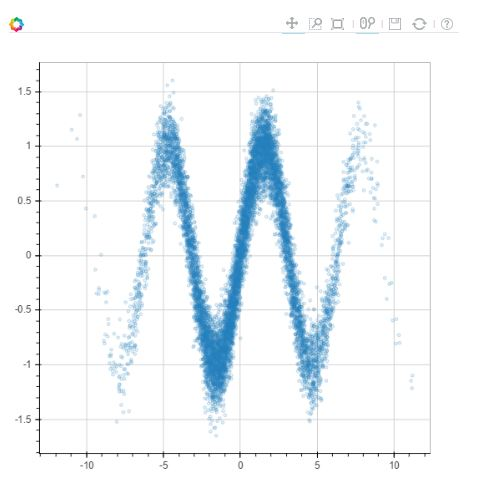
\includegraphics[width=0.7\linewidth]{images/06-WebGL-01}

\end{figure}
\newpage
\begin{framed}
	\begin{verbatim}
import numpy as np

from bokeh.plotting import figure, show, output_file

N = 10000

x = np.random.normal(0, np.pi, N)
y = np.sin(x) + np.random.normal(0, 0.2, N)

output_file("scatter10k.html", title="scatter 10k points (with WebGL)")

p = figure(webgl=True)
p.scatter(x,y, alpha=0.1)
show(p)
	
\end{verbatim}
\end{framed}
\begin{figure}
\centering
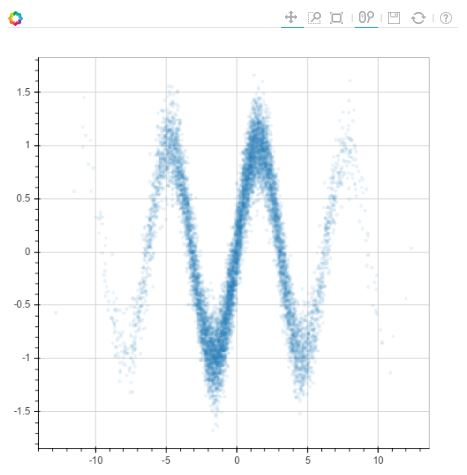
\includegraphics[width=0.7\linewidth]{images/06-WebGL-02}
\end{figure}

\end{document}